\label{research}
So far, we discussed an extension of the pilot abstraction to support data analytics and task based data intensive applications on HPC resources, a comparison between different task-based data oriented frameworks, and a design comparison for scientific workflows.
In addition, we identified a need for the execution of scientific computational campaigns with minimum user intervention, independent from users' scientific domain.
In this section, we motivate and propose a Campaign Manager (CM) for creating and enacting a campaign execution plan. \mtnote{Do we need to explain how these three topics fit together?}


\subsection{Proposed Topic}
%Campaigns from the biomolecular and earth sciences are diverse in terms of composition, number and size of workflow members, and dynamicity. \mtnote{What does ``composition'' stand for in this context?}
%Biomolecular science campaigns may be comprised of a small number of workflows with millions of tasks, or thousands of workflows with tens to hundreds tasks~\cite{dakka2018high}. \mtnote{And everything in between these two boundaries?}
%Earth sciences campaigns, especially those which use VHR \mtnote{expand if not used before} satellite imagery, comprise of workflows with thousands of tasks.
%The number of workflows depends on the number of images the user has access to as well as the time they are able to obtain imagery.
%These workflows can be static~\cite{paraskevakos2019workflow} or dynamic~\cite{dakka2018high}. \mtnote{Did we explained why campaigns from these two science domains are interesting for this proposal?}

% ------------------------------------------------------------------------------
% Scientific campaings
Scientific workflows are generally described by direct acyclic graphs (DAG), where the nodes are tasks and the edges are dependencies.
A subset of this general description of workflows are those which can be represented via the Pipeline, Stage, Task (PST) model~\cite{balasubramanian2018harnessing}.
The PST model describes workflows as a set of pipelines, where each pipeline is a sequence of stages.
Each stage then is a set of tasks that need to be executed.
Concurrency is achieved at the level of pipelines and the level of tasks. 
Based on our use cases, we are particularly interested in scientific campaigns comprised by workflows that can be described via the PST model. \mtnote{Why?}
Figure~\ref{fig:bio_earth_workflows} shows two example workflows from the biomolecular sciences (Fig.~\ref{fig:bio_workflow}) and the earth sciences (Fig.~\ref{fig:earth_workflow}). 

\begin{figure*}[ht!]
    \centering
    \begin{subfigure}[b]{0.45\textwidth}
        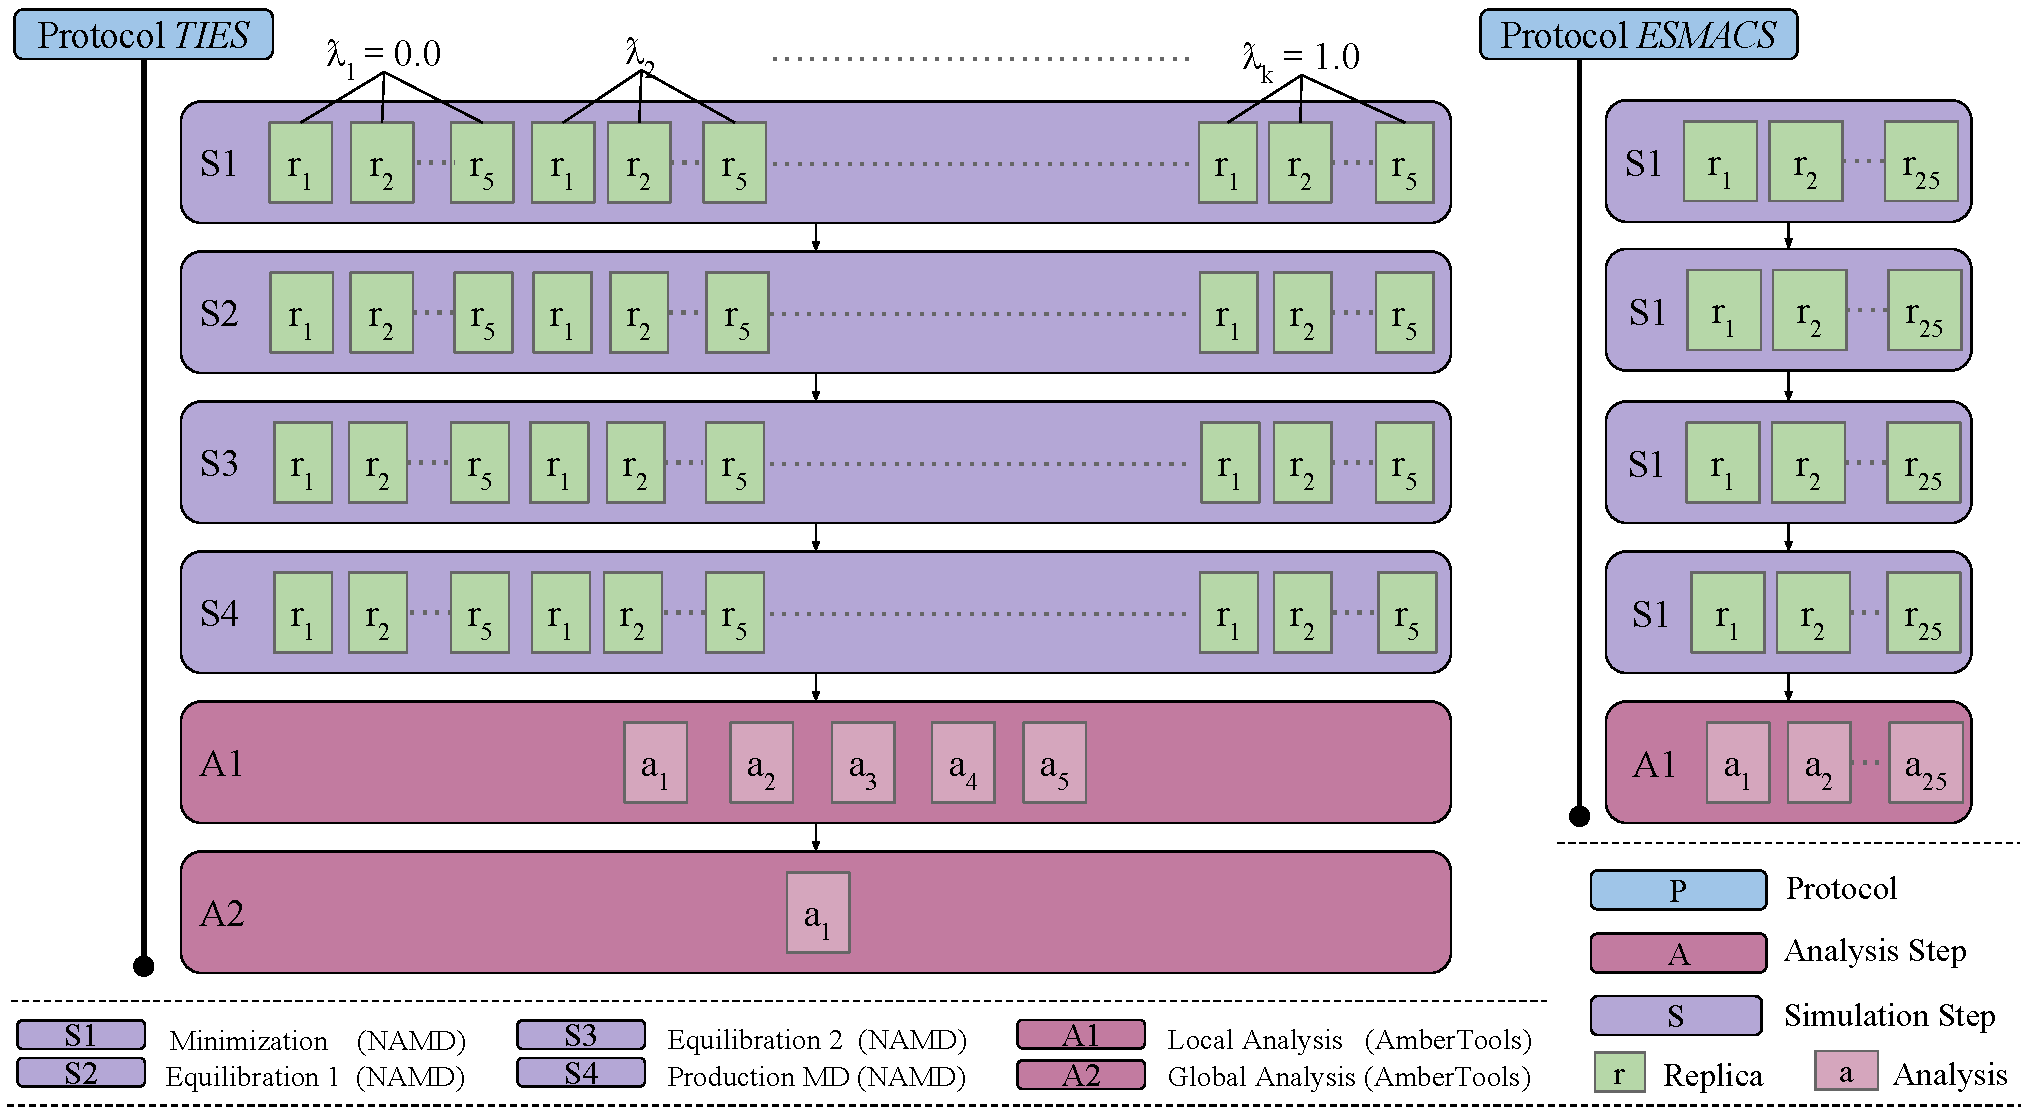
\includegraphics[width=\linewidth]{figures/bio_workflow.pdf}
        \caption{}
        \label{fig:bio_workflow}
    \end{subfigure}%
    ~ 
    \begin{subfigure}[b]{0.45\textwidth}
        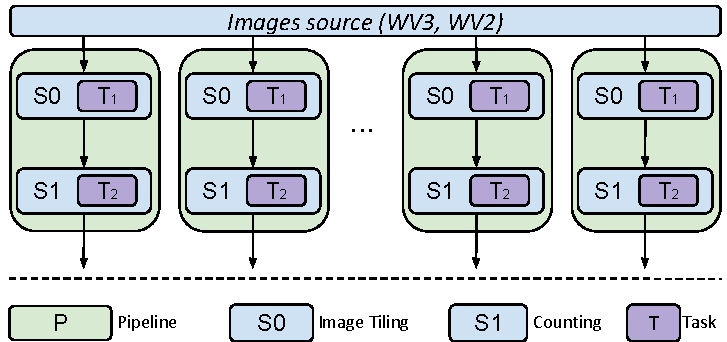
\includegraphics[width=\linewidth]{figures/earth_workflow.pdf}
        \caption{}
        \label{fig:earth_workflow}
    \end{subfigure}
    \caption{Biomolecular and Earth Science example workflows. \ref{fig:bio_workflow} Biomolecular workflow based on PST model example~\cite{dakka2018concurrent}; \ref{fig:earth_workflow} Earth science workflow based on PST model example~\cite{paraskevakos2019workflow}}\label{fig:bio_earth_workflows}
\end{figure*}

Resource requirements of \mtnote{which ones?} campaigns are heterogeneous, in terms of number of resources required and type. 
Biomolecular science software tools support MPI/OpenMP, GPUs, and other accelerators, such as Intel Phi processors~\cite{cheatham2015impact} for executing either physical systems simulations or trajectory data analysis. \mtnote{simulations of? Analysis of?}
In addition, some biomolecular analysis tool require data oriented frameworks, such as Parallel MDAnalysis~\cite{fan2019pmda}\mtnote{expand acronym, add other examples.}.
Earth sciences applications, based on imagery, use workflows that execute a series of CPU based preprocessing, and eventually execute a computer vision algorithm on GPUs~\cite{paraskevakos2019workflow}\mtnote{This is specific to the applications you worked on, not necessarely true for all workflows used by the earth sciences communities. This comment seems to apply also to all the other examples of this paragraph}.

HPC resource are dynamic in nature, as their availability is subject to a broad spectrum of policies.
These policies determine:
\begin{inparaenum}[1)]
\item the maximum number of resources and walltime a user can request concurrently in a single request,
\item the maximum number of concurrently submitted or active requests, and
\item one or more usage charging models, which determine the total amount or resources the has access to.
\end{inparaenum}

%The makespan of a campaign can be \mtnote{missing verb: derived maybe?} from a simple arithmetics calculation to a complex problem, depending on the heterogeneity of the campaign's workflows, maximum concurrency and resource dynamicity. \mtnote{This seems to assume that the reader has to understand the relation between makespan, heterogeneity and dynamicity on her own. I would refine and explain better.}
%Workflows can be heterogeneous in space, i.e., the number of tasks and resource requirements, and in time, i.e., the execution time needed to execute.
%When workflows are the same in space and time, they are considered homogeneous.
%Assuming enough resources to execute a workflow, when a campaign consists of homogeneous workflows any order of workflow execution would provide the same makespan. 
%When heterogeneity is introduced, randomly ordering the workflows' execution provides different makespan for different instances of the ordering.
%This is especially true, when there are not enough resources to execute all the workflows concurrently.
%As a result, calculating the makespan of the campaign based on workflow order execution becomes important to decide whether the selected mapping satisfies or not the campaign's computational campaign \mtnote{``campaign's computational campaign'' makes no sense.}.

\mtnote{This seems to assume that the reader has to understand the relation between makespan, heterogeneity and dynamicity on her own. I would refine and explain better.}\gpnote{Broke it into two paragraphs.}
Several factor can influence the complexity of calculating the makespan of a campaign, such as heterogeneity of the campaign's workflows, concurrency and resource dynamicity.
Workflows can be heterogeneous in space, i.e., the number of tasks and resource requirements, and in time, i.e., the execution time needed to execute.
When workflows are the same in space and time, they are considered homogeneous.
Assuming homogeneous workflows and a single static resource, the makespan of the campaign is equal to the addition of the execution time of all workflows.
When workflows from the campaign can be executed concurrently on static resources, the makespan of the campaign is equal to rounding up the division of the number of workflows to the number of resources times the execution time of a single workflow.
Dynamic resources can influence the makespan, since they will affect the maximum number of workflows that were executed serially in a resource.
As a result, any order of executing the workflows of a campaign produces the same makespan, which also is the minimum makespan.

When workflows are heterogeneous, the level of concurrency, resource dynamicity, and workflow execution order can affect the makespan.
In the case of sequential execution of the workflows, the order of the execution does not affect the makespan of the campaign.
When concurrency is introduced, the order and placing of workflows can affect the makespan of the campaign.
For example, a campaign has 9 heterogeneous in time workflows with sorted execution times from 1 to 9 time units, and they can be executed on three resources.
A possible execution order would be to place three consecutive workflows to each resource.
The makespan would be equal to the summation of the execution time of last workflows, i.e. $7 + 8 + 9 = 24$ time units.
Instead, executing the three workflows with the largest concurrently and position new workflows to resources as they become available, it can produce a makespan of $16$ time units.
This problem becomes complicated when the number of workflows in the campaign is in the order of thousands.
Workflows are heterogeneous in size, and as a consequence multiple workflows may fit in a single resource.
Grouping multiple workflows together to execute as a single workflow may further reduce the campaigns makespan.
As a result, calculating the makespan of the campaign for based on workflow stacking, execution order, and workflow to resource mapping becomes important.
The combination of workflow stacking, execution order, and workflow to resource mapping that produces a makespan which satisfies the computational objective of the campaign is the execution plan of the campaign.

% ----------------------------------------------------------------------------
% campaign makespan modeling
We propose to initially utilize and extend the Heterogeneous Earliest Finish Time (HEFT)~\cite{topcuoglu2002performance} algorithm \mtnote{for doing what?}.
HEFT is an offline scheduling algorithm which calculates the makespan of a workflow on heterogeneous resources.
HEFT uses a matrix to represent execution time of tasks on resources, assigning tasks to the resource that minimizes the finish time of the task, and has complexity proportional to the number of dependencies between tasks and the number of resources offered \mtnote{Why suddenly are we writing about tasks? What is the relationship between HEFT, tasks, workflows and campaigns?}
Furthermore, there has been some initial research to extend HEFT to resources that provide CPU and GPUs~\cite{shetti2013optimization}, as well as a HEFT extension on dynamic resources~\cite{dong2007pfas}.

There are several alternative methods and algorithms to calculate and optimize the makespan of a workflow~\cite{lu2019review}, including queuing networks~\cite{yao2019throughput,bao2019performance}, domain specific languages~\cite{carothers2017durango,maheshwari2016workflow}, and machine learning~\cite{witt2019predictive,pumma2017runtime}.
Queuing networks will be of limited use because they require from the user to provide a queuing network equivalent of the campaign.
As a result, having the user provide a queuing network representation of the campaign adds an additional layer of complexity. \mtnote{These two sentences are unclear, please revise.}
Domain specific languages would require too much engineering effort to convert a workflow representation based on domain specific assumptions, e.g., MPI style workflow, or specific languages representation, e.g., Swift, to a PST model representation \mtnote{This is unconvincing: we choose to use the PST model and then we say that it requires too much effort? Remember: the argumentation here has to be `scientific', not just based on 'I want to use EnTK so this would require too much time'.}.
Machine Learning approaches would require model training, validation and testing to produce a model \mtnote{Why would this be a problem?}.
In addition, since the execution is done on dynamic resources, the model should be retrained after every workflow execution.

% ----------------------------------------------------------------------------
% Initial Assumptions
We propose to extend HEFT to support execution of a computational campaign on dynamic resources \mtnote{and heterogeneous?}.
When executing a workflows HEFT assumes that any available resource can execute the workflow's tasks \mtnote{Why this statement is relevant?}.
In addition, when executing a workflow on HPC resources, it can be assumed that all the resources will be available during the execution of the workflows \mtnote{Explain further, you seem to be assuming the reader understand a lot of implications of what you are writing. This is generally untrue has the reader has a very different background from yours and never thought to what you are writing here before.}.
These two assumptions are not necessarily true when a computational campaign is executed.
As campaign's workflows are heterogeneous, not all resources will satisfy the space requirements for all the workflows \mtnote{why?}.
Introducing resource dynamicity requires HEFT to take into account resource availability to decide on which resources it will schedule workflows.
In addition, it should update the schedule as resources become unavailable.

% ----------------------------------------------------------------------------
% Campaign Manager definition, requirements, features and capabilities
We propose to design a campaign manager (CM) which, given a campaign, an objective, and a set of constraints, can derive an execution plan by utilizing the proposed makespan HEFT method.
Execution planning for workflows are provided by Pegasus~\cite{deelman2015pegasus}, and ASKALON~\cite{fahringer2005askalon} \mtnote{only these two among all the existing systems? Please refine and expand, explaining that these are just examples. Also, expand appropriately introducing the notions of planning and plan and explaining why they relate to campaign management.}.
We propose to extend these capability to campaigns.

Figure~\ref{fig:refarch} shows a reference architecture where the CM has two sub-components:
\begin{inparaenum}[(1)]
\item Makespan Calculator which implements HEFT, and
\item an Executor which executes the plan. 
\end{inparaenum}
Workflow execution will be done through an existing workflow management framework (WMF) on HPC resources.
If necessary, CM will adapt the execution plan by updating the workflows to resource mapping decisions. 
These updates will be based on workflows execution metrics provided by the selected WMF such as tasks execution time, overheads calculation and time to completion.
These metrics will be aggregated across workflows resulting in campaign-wide execution metrics.

\begin{figure*}[t]
    \centering
    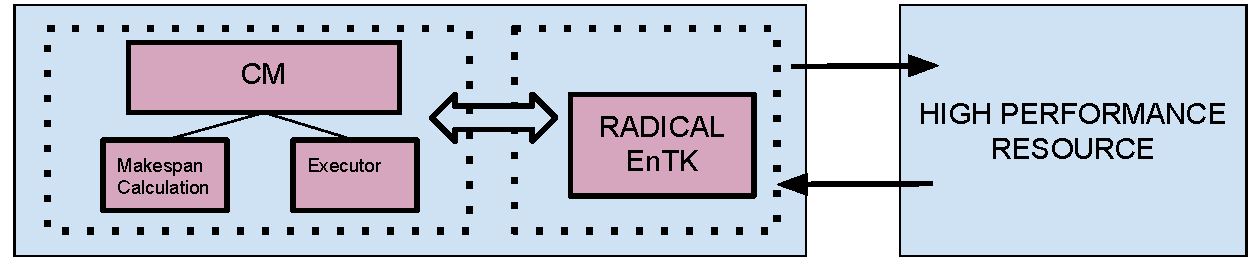
\includegraphics[width=.95\textwidth]{figures/CEM_RefArch.pdf}
    \caption{Reference Architecture of a Campaign Manager. Basic 
    subcomponents of Campaign Manager (CM): 1) Makespan Calculation, and 2) Executor. 
    CM communicates decisions to RADICAL-EnTK. CM communicates with HPCs to 
    execute parts of the campaign.}\label{fig:refarch}
\end{figure*}

The Makespan Calculator will be responsible for calculating and optimizing \mtnote{is it a calculator or an optimizer? Seem different capabilities to me and not necessarely part of the same component} the makespan of a campaign based on a set of resources, and the objective.
The calculator will utilize the extend HEFT algorithm to derive an execution plan of the campaign. \mtnote{It seems to me that makespan calculation is only one of the elements needed to derive a plan. As such, I think you need at least two components in your architecture: makespan calculator and planner.}
In addition, the Campaign Manager \mtnote{are we describing the Makespan Calculator or the Campaign Manager} should be able to verify whether a resource is available and update the plan accordingly.

The Executor sub-component is responsible to execute and monitor the plan \mtnote{where is the plan coming from?} by interfacing with a WMF.
Based on the plan the Makespan calculator decided, the Executor submits workflows to a WMF to execute on the selected resource.
This requires the Executor to work upon multiple workflows concurrently \mtnote{and why is this important?}.
In addition, it should monitor workflow execution and resource availability \mtnote{why?}.
An important requirement for the executor is to identify the reason of a failing workflow.
When the failure is because the resource is not available, the specific workflow may need to be rescheduled and the plan to be updated.

RADICAL-Ensemble Toolkit~\cite{balasubramanian2018harnessing} (EnTK) is a workflow management framework.
We selected to utilize EnTK because it fits the requirements of the target use cases.
EnTK defines workflows as a set of pipelines, each pipeline is a sequence of stages, and in turn each stage a set of tasks.
EnTK support the execution of a sequence of workflows may either reuse resources or request new ones, based on how the user has programmed the application \mtnote{grammar: from `may' onwards I do not understand the sentence anymore.}.
EnTK workflow execution is stateful, provides execution metrics, such as task execution time, and supports workflow execution on multiple HPC resources.
Furthermore, EnTK supports a pilot runtime system, RADICAL-Pilot~\cite{merzky2019using}, to execute workflows on HPC resources.
Pilot systems submit job placeholders on resources, and are able to execute tasks on the acquired resources.
In addition, the specifics of each individual resource is abstracted and hidden from the upper layer.
As a result, the campaign manager will see a set of resources where workflows should be executed upon \mtnote{not sure  understand how this follows from your explanation of pilots.}.
The proposed campaign manager will interface with EnTK to execute workflows based on a derived execution plan.


Initially, we will assume a static campaign with static heterogeneous workflows, executing on static resources.
This will allow us to understand the selected algorithm \mtnote{what algorithm? For doing what?}, and find its performance compared to a random plan.
Next, we will relax the assumption of static resources and work with dynamic resources.
We will introduce resource dynamicity as resource availability, where resources will not be available and the plan would have to be adjusted.

\mtnote{General note: this needs to be expanded following the comments I left. At the moment, a lot of this still reads as a set of sometimes disconnected statements. We need to iterate so to produced a more detailed description of the research you propose to conduct in the next year, a description backed by existing literature and your own argumentation. From our discussions, I know you have the material needed to iterate this initial draft. }
